\documentclass[dvipsnames]{article}
\usepackage[english]{babel}
\usepackage{multirow}
\usepackage[letterpaper,top=2cm,bottom=2cm,left=3cm,right=3cm,marginparwidth=1.75cm]{geometry}
\usepackage{amsmath}
\usepackage{graphicx}
\usepackage{minted}
\usepackage{amsthm}
\usepackage{mathtools}
\usepackage[colorlinks=true, allcolors=blue]{hyperref}
\usepackage{fancyhdr}
\usepackage{enumerate}

\usepackage{tikz}
\usetikzlibrary{shapes}
\usetikzlibrary{arrows}

\tikzset{
  treenode/.style = {align=center, inner sep=0pt, text centered,
    font=\sffamily},
  avl_node/.style = {treenode, circle, black, draw=black,
    text width=1.5em, very thick},% arbre rouge noir, noeud rouge
  black_node/.style = {treenode, circle, white, font=\sffamily\bfseries, draw=black,
    fill=black, text width=1.5em},% arbre rouge noir, noeud noir
  red_node/.style = {treenode, circle, red, draw=red,
    text width=1.5em, very thick},% arbre rouge noir, noeud rouge
  nil_leaf/.style = {treenode, rectangle, draw=black, fill=black,
    minimum width=0.3em, minimum height=0.3em}% arbre rouge noir, nil
}

\begin{document}
\section*{Week 8. Problem set (solutions by \textcolor{blue}{Karim Khabibrakhmanov})}

\thispagestyle{fancy}
\lhead{Karim Khabibrakhmanov (\texttt{k.khabibrakhmanov@innopolis.university}), group B24-DSAI-05}

\begin{enumerate}
  \item Perform \textsc{Heap-Sort}~\cite[\S 6.4]{Cormen2022} on the following input array:
  \begin{center}
  \begin{tabular}{|c|c|c|c|c|c|c|c|c|c|c|c|c|c|c|}
    \hline
      \makebox[\widthof{0}][c]{2}
    & \makebox[\widthof{0}][c]{3}
    & \makebox[\widthof{0}][c]{0}
    & \makebox[\widthof{0}][c]{4}
    & \makebox[\widthof{0}][c]{7}
    & \makebox[\widthof{0}][c]{1}
    & \makebox[\widthof{0}][c]{5}
    & \makebox[\widthof{0}][c]{8}
    & \makebox[\widthof{0}][c]{6}
    \\
    \hline
  \end{tabular}
  \end{center}

  Show the state of the array after each call to \textsc{Max-Heapify} from the \textsc{Heap-Sort} procedure
  (solution must have 8 arrays).

    \color{blue}
    \textbf{Answer:}\\Initially, we need to apply \textsc{Max-Heapify} to our array. Here is our resulting array:
    \begin{center}
    \begin{tabular}{|c|c|c|c|c|c|c|c|c|c|c|c|c|c|c|}
    \hline
      \makebox[\widthof{0}][c]{8}
    & \makebox[\widthof{0}][c]{7}
    & \makebox[\widthof{0}][c]{5}
    & \makebox[\widthof{0}][c]{6}
    & \makebox[\widthof{0}][c]{2}
    & \makebox[\widthof{0}][c]{1}
    & \makebox[\widthof{0}][c]{0}
    & \makebox[\widthof{0}][c]{3}
    & \makebox[\widthof{0}][c]{4}
    \\
    \hline
  \end{tabular}
  \end{center}
  \\Next, for all other arrays, we apply an algorithm that will swap the first and last elements of the array. After that, we re-apply \textsc{Max-Heapify}:
  \begin{center}
  \\1:
  \begin{tabular}{|c|c|c|c|c|c|c|c|c|c|c|c|c|c|c|}
    \hline
      \makebox[\widthof{0}][c]{7}
    & \makebox[\widthof{0}][c]{6}
    & \makebox[\widthof{0}][c]{5}
    & \makebox[\widthof{0}][c]{4}
    & \makebox[\widthof{0}][c]{2}
    & \makebox[\widthof{0}][c]{1}
    & \makebox[\widthof{0}][c]{0}
    & \makebox[\widthof{0}][c]{3}
    & \makebox[\widthof{0}][c]{8}
    \\
    \hline
  \end{tabular}
  \\2:
  \begin{tabular}{|c|c|c|c|c|c|c|c|c|c|c|c|c|c|c|}
    \hline
      \makebox[\widthof{0}][c]{6}
    & \makebox[\widthof{0}][c]{4}
    & \makebox[\widthof{0}][c]{5}
    & \makebox[\widthof{0}][c]{3}
    & \makebox[\widthof{0}][c]{2}
    & \makebox[\widthof{0}][c]{1}
    & \makebox[\widthof{0}][c]{0}
    & \makebox[\widthof{0}][c]{7}
    & \makebox[\widthof{0}][c]{8}
    \\
    \hline
  \end{tabular}
  \\ 3:
  \begin{tabular}{|c|c|c|c|c|c|c|c|c|c|c|c|c|c|c|}
    \hline
      \makebox[\widthof{0}][c]{5}
    & \makebox[\widthof{0}][c]{4}
    & \makebox[\widthof{0}][c]{1}
    & \makebox[\widthof{0}][c]{3}
    & \makebox[\widthof{0}][c]{2}
    & \makebox[\widthof{0}][c]{0}
    & \makebox[\widthof{0}][c]{6}
    & \makebox[\widthof{0}][c]{7}
    & \makebox[\widthof{0}][c]{8}
    \\
    \hline
  \end{tabular}
  \\ 4:
  \begin{tabular}{|c|c|c|c|c|c|c|c|c|c|c|c|c|c|c|}
    \hline
      \makebox[\widthof{0}][c]{4}
    & \makebox[\widthof{0}][c]{3}
    & \makebox[\widthof{0}][c]{1}
    & \makebox[\widthof{0}][c]{0}
    & \makebox[\widthof{0}][c]{2}
    & \makebox[\widthof{0}][c]{5}
    & \makebox[\widthof{0}][c]{6}
    & \makebox[\widthof{0}][c]{7}
    & \makebox[\widthof{0}][c]{8}
    \\
    \hline
  \end{tabular}
  \\ 5:
  \begin{tabular}{|c|c|c|c|c|c|c|c|c|c|c|c|c|c|c|}
    \hline
      \makebox[\widthof{0}][c]{3}
    & \makebox[\widthof{0}][c]{2}
    & \makebox[\widthof{0}][c]{1}
    & \makebox[\widthof{0}][c]{0}
    & \makebox[\widthof{0}][c]{4}
    & \makebox[\widthof{0}][c]{5}
    & \makebox[\widthof{0}][c]{6}
    & \makebox[\widthof{0}][c]{7}
    & \makebox[\widthof{0}][c]{8}
    \\
    \hline
  \end{tabular}
  \\ 6:
  \begin{tabular}{|c|c|c|c|c|c|c|c|c|c|c|c|c|c|c|}
    \hline
      \makebox[\widthof{0}][c]{2}
    & \makebox[\widthof{0}][c]{0}
    & \makebox[\widthof{0}][c]{1}
    & \makebox[\widthof{0}][c]{3}
    & \makebox[\widthof{0}][c]{4}
    & \makebox[\widthof{0}][c]{5}
    & \makebox[\widthof{0}][c]{6}
    & \makebox[\widthof{0}][c]{7}
    & \makebox[\widthof{0}][c]{8}
    \\
    \hline
  \end{tabular}
  \\ 7:
  \begin{tabular}{|c|c|c|c|c|c|c|c|c|c|c|c|c|c|c|}
    \hline
      \makebox[\widthof{0}][c]{1}
    & \makebox[\widthof{0}][c]{0}
    & \makebox[\widthof{0}][c]{2}
    & \makebox[\widthof{0}][c]{3}
    & \makebox[\widthof{0}][c]{4}
    & \makebox[\widthof{0}][c]{5}
    & \makebox[\widthof{0}][c]{6}
    & \makebox[\widthof{0}][c]{7}
    & \makebox[\widthof{0}][c]{8}
    \\
    \hline
  \end{tabular}
  \\ 8:
  \begin{tabular}{|c|c|c|c|c|c|c|c|c|c|c|c|c|c|c|}
    \hline
      \makebox[\widthof{0}][c]{0}
    & \makebox[\widthof{0}][c]{1}
    & \makebox[\widthof{0}][c]{2}
    & \makebox[\widthof{0}][c]{3}
    & \makebox[\widthof{0}][c]{4}
    & \makebox[\widthof{0}][c]{5}
    & \makebox[\widthof{0}][c]{6}
    & \makebox[\widthof{0}][c]{7}
    & \makebox[\widthof{0}][c]{8}
    \\
    \hline
  \end{tabular}
  \end{center}
  \\Finally sorted array using \textsc{Heap-Sort}:
  \begin{tabular}{|c|c|c|c|c|c|c|c|c|c|c|c|c|c|c|}
    \hline
      \makebox[\widthof{0}][c]{0}
    & \makebox[\widthof{0}][c]{1}
    & \makebox[\widthof{0}][c]{2}
    & \makebox[\widthof{0}][c]{3}
    & \makebox[\widthof{0}][c]{4}
    & \makebox[\widthof{0}][c]{5}
    & \makebox[\widthof{0}][c]{6}
    & \makebox[\widthof{0}][c]{7}
    & \makebox[\widthof{0}][c]{8}
    \\
    \hline
  \end{tabular}
    \color{black}
    \item
    A $d$-ary heap is similar to a binary heap, except non-leaf nodes have $d$ children instead of $2$ children (except the last non-leaf node, which is allowed to have fewer children).
    Adjust the array representation and the efficient implementations of \textsc{Max-Heapify} and \textsc{Build-Max-Heap}.
    \textbf{Write down} the generalized pseudocode of \textsc{Max-Heapify} and \textsc{Build-Max-Heap} for $d$-ary heaps for any $d$.

    \color{blue}
    \textbf{Pseudocode:}
        \begin{minted}[linenos,escapeinside=||]{python}
    Max-Heapify(A, i, d):
        maximum = i
        for k = 1 to d:
            child = d * i + k
            if child < A.size() and A[child] > A[maximum]:
                maximum = child
        if maximum != i:
            swap(A[i], A[maximum])
            Max-Heapify(A, maximum, d)        
    
    Build-Max-Heap(A, d):
        for i = ((A.size() - 1) / d) to 0:
            Max-Heapify(A, i, d)
\end{minted}
    \color{black}

    Then, perform a variation of \textsc{Heap-Sort}~\cite[\S 6.4]{Cormen2022} using a 4-ary heap on the following input array:
    
  
    \begin{center}
    \begin{tabular}{|c|c|c|c|c|c|c|c|c|c|c|c|c|c|c|}
      \hline
        \makebox[\widthof{0}][c]{2}
      & \makebox[\widthof{0}][c]{3}
      & \makebox[\widthof{0}][c]{0}
      & \makebox[\widthof{0}][c]{4}
      & \makebox[\widthof{0}][c]{7}
      & \makebox[\widthof{0}][c]{1}
      & \makebox[\widthof{0}][c]{5}
      & \makebox[\widthof{0}][c]{8}
      & \makebox[\widthof{0}][c]{6}
      \\
      \hline
    \end{tabular}
    \end{center}
  
    \textbf{Show} the state of the array after each call to \textsc{Max-Heapify} from the \textsc{Heap-Sort} procedure
    (solution must contain 8 arrays and the pseudocode for generalized \textsc{Max-Heapify} and \textsc{Build-Max-Heap}).

    \color{blue}
    \textbf{Answer:}\\Initially, we need to apply \textsc{Max-Heapify} to our array. Here is our resulting array:
    \begin{center}
    \begin{tabular}{|c|c|c|c|c|c|c|c|c|c|c|c|c|c|c|}
    \hline
      \makebox[\widthof{0}][c]{8}
    & \makebox[\widthof{0}][c]{6}
    & \makebox[\widthof{0}][c]{0}
    & \makebox[\widthof{0}][c]{4}
    & \makebox[\widthof{0}][c]{7}
    & \makebox[\widthof{0}][c]{1}
    & \makebox[\widthof{0}][c]{5}
    & \makebox[\widthof{0}][c]{3}
    & \makebox[\widthof{0}][c]{2}
    \\
    \hline
  \end{tabular}
  \end{center}
    \\Next, for all other arrays, we apply an algorithm that will swap the first and last elements of the array. After that, we re-apply \textsc{Max-Heapify}:
  \begin{center}
  \\1:
  \begin{tabular}{|c|c|c|c|c|c|c|c|c|c|c|c|c|c|c|}
    \hline
      \makebox[\widthof{0}][c]{7}
    & \makebox[\widthof{0}][c]{6}
    & \makebox[\widthof{0}][c]{0}
    & \makebox[\widthof{0}][c]{4}
    & \makebox[\widthof{0}][c]{2}
    & \makebox[\widthof{0}][c]{1}
    & \makebox[\widthof{0}][c]{5}
    & \makebox[\widthof{0}][c]{3}
    & \makebox[\widthof{0}][c]{8}
    \\
    \hline
  \end{tabular}
  \\2:
  \begin{tabular}{|c|c|c|c|c|c|c|c|c|c|c|c|c|c|c|}
    \hline
    \makebox[\widthof{0}][c]{6}
    & \makebox[\widthof{0}][c]{5}
    & \makebox[\widthof{0}][c]{0}
    & \makebox[\widthof{0}][c]{4}
    & \makebox[\widthof{0}][c]{2}
    & \makebox[\widthof{0}][c]{1}
    & \makebox[\widthof{0}][c]{3}
    & \makebox[\widthof{0}][c]{7}
    & \makebox[\widthof{0}][c]{8}
    \\
    \hline
  \end{tabular}
  \\ 3:
  \begin{tabular}{|c|c|c|c|c|c|c|c|c|c|c|c|c|c|c|}
    \hline
      \makebox[\widthof{0}][c]{5}
    & \makebox[\widthof{0}][c]{3}
    & \makebox[\widthof{0}][c]{0}
    & \makebox[\widthof{0}][c]{4}
    & \makebox[\widthof{0}][c]{2}
    & \makebox[\widthof{0}][c]{1}
    & \makebox[\widthof{0}][c]{6}
    & \makebox[\widthof{0}][c]{7}
    & \makebox[\widthof{0}][c]{8}
    \\
    \hline
  \end{tabular}
  \\ 4:
  \begin{tabular}{|c|c|c|c|c|c|c|c|c|c|c|c|c|c|c|}
    \hline
      \makebox[\widthof{0}][c]{4}
    & \makebox[\widthof{0}][c]{3}
    & \makebox[\widthof{0}][c]{0}
    & \makebox[\widthof{0}][c]{1}
    & \makebox[\widthof{0}][c]{2}
    & \makebox[\widthof{0}][c]{5}
    & \makebox[\widthof{0}][c]{6}
    & \makebox[\widthof{0}][c]{7}
    & \makebox[\widthof{0}][c]{8}
    \\
    \hline
  \end{tabular}
  \\ 5:
  \begin{tabular}{|c|c|c|c|c|c|c|c|c|c|c|c|c|c|c|}
    \hline
      \makebox[\widthof{0}][c]{3}
    & \makebox[\widthof{0}][c]{2}
    & \makebox[\widthof{0}][c]{0}
    & \makebox[\widthof{0}][c]{1}
    & \makebox[\widthof{0}][c]{4}
    & \makebox[\widthof{0}][c]{5}
    & \makebox[\widthof{0}][c]{6}
    & \makebox[\widthof{0}][c]{7}
    & \makebox[\widthof{0}][c]{8}
    \\
    \hline
  \end{tabular}
  \\ 6:
  \begin{tabular}{|c|c|c|c|c|c|c|c|c|c|c|c|c|c|c|}
    \hline
      \makebox[\widthof{0}][c]{2}
    & \makebox[\widthof{0}][c]{1}
    & \makebox[\widthof{0}][c]{0}
    & \makebox[\widthof{0}][c]{3}
    & \makebox[\widthof{0}][c]{4}
    & \makebox[\widthof{0}][c]{5}
    & \makebox[\widthof{0}][c]{6}
    & \makebox[\widthof{0}][c]{7}
    & \makebox[\widthof{0}][c]{8}
    \\
    \hline
  \end{tabular}
  \\ 7:
  \begin{tabular}{|c|c|c|c|c|c|c|c|c|c|c|c|c|c|c|}
    \hline
      \makebox[\widthof{0}][c]{1}
    & \makebox[\widthof{0}][c]{0}
    & \makebox[\widthof{0}][c]{2}
    & \makebox[\widthof{0}][c]{3}
    & \makebox[\widthof{0}][c]{4}
    & \makebox[\widthof{0}][c]{5}
    & \makebox[\widthof{0}][c]{6}
    & \makebox[\widthof{0}][c]{7}
    & \makebox[\widthof{0}][c]{8}
    \\
    \hline
  \end{tabular}
  \\ 8:
  \begin{tabular}{|c|c|c|c|c|c|c|c|c|c|c|c|c|c|c|}
    \hline
      \makebox[\widthof{0}][c]{0}
    & \makebox[\widthof{0}][c]{1}
    & \makebox[\widthof{0}][c]{2}
    & \makebox[\widthof{0}][c]{3}
    & \makebox[\widthof{0}][c]{4}
    & \makebox[\widthof{0}][c]{5}
    & \makebox[\widthof{0}][c]{6}
    & \makebox[\widthof{0}][c]{7}
    & \makebox[\widthof{0}][c]{8}
    \\
    \hline
  \end{tabular}
  \end{center}
  \\Finally sorted array using \textsc{Heap-Sort}:
  \begin{tabular}{|c|c|c|c|c|c|c|c|c|c|c|c|c|c|c|}
    \hline
      \makebox[\widthof{0}][c]{0}
    & \makebox[\widthof{0}][c]{1}
    & \makebox[\widthof{0}][c]{2}
    & \makebox[\widthof{0}][c]{3}
    & \makebox[\widthof{0}][c]{4}
    & \makebox[\widthof{0}][c]{5}
    & \makebox[\widthof{0}][c]{6}
    & \makebox[\widthof{0}][c]{7}
    & \makebox[\widthof{0}][c]{8}
    \\
    \hline
  \end{tabular}
    \color{black}
  
    \item
    Insert the $\langle \mathsf{key}, \mathsf{value} \rangle$ items
    into an empty B-tree~\cite[\S 18]{Cormen2022} with minimum degree $t = 2$:
  
    \begin{enumerate}
      \item $\langle 32, I \rangle,
          \; \langle 17, I \rangle,
          \; \langle 9, X \rangle,
          \; \langle 21, C \rangle,
          \; \langle 11, E \rangle$
      \item $\langle 2, A \rangle,
          \; \langle 28, E \rangle,
          \; \langle 36, G \rangle,
          \; \langle 3, E \rangle,
          \; \langle 4, T \rangle$
      \item $\langle 18, B \rangle,
          \; \langle 13, E \rangle,
          \; \langle 6, T \rangle,
          \; \langle 7, R \rangle,
          \; \langle 37, I \rangle$
      \item $\langle 26, L \rangle,
          \; \langle 33, N \rangle,
          \; \langle 20, U \rangle,
          \; \langle 24, I \rangle,
          \; \langle 30, D \rangle$
    \end{enumerate}
  
    Show the state of the tree after every 5 insertions.
    Depict each tree as a sequence of arrays for each layer.
    For example, consider this B-tree:
  
    \begin{center}
    \footnotesize
    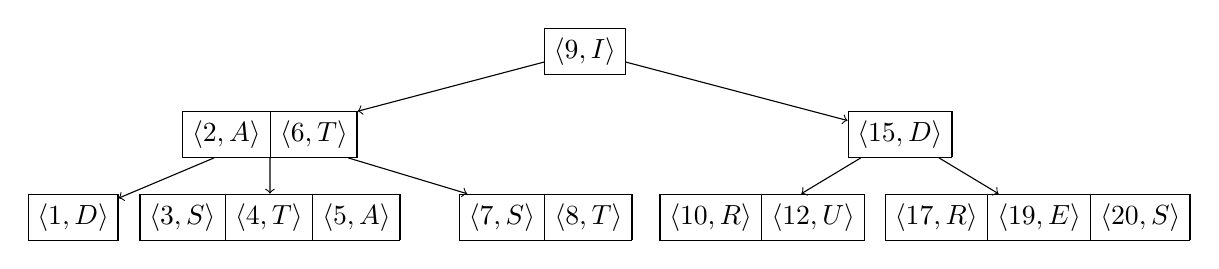
\begin{tikzpicture}[level distance=30pt]
    \tikzstyle{bplus}=[rectangle split, rectangle split horizontal,rectangle split ignore empty parts,draw]
    \tikzstyle{every node}=[bplus]
    \tikzstyle{level 1}=[sibling distance=80mm]
    \tikzstyle{level 2}=[sibling distance=35mm]
    \node {$\langle 9, I \rangle$} [->]
      child {node {$\langle 2, A \rangle$ \nodepart{two} $\langle 6, T \rangle$}
        child[sibling distance=25mm] {node {$\langle 1, D \rangle$}}
        child {node {$\langle 3, S\rangle$ \nodepart{two} $\langle 4, T\rangle$ \nodepart{three} $\langle 5, A\rangle$}}
        child {node {$\langle 7, S\rangle$ \nodepart{two} $\langle 8, T\rangle$}}
      }
      child {node {$\langle 15, D \rangle$}
        child {node {$\langle 10, R \rangle$ \nodepart{two} $\langle 12, U \rangle$}}
        child {node {$\langle 17, R\rangle$ \nodepart{two} $\langle 19, E\rangle$ \nodepart{three} $\langle 20, S\rangle$}}
      }
    ;\end{tikzpicture}
    \end{center}
  
    The tree above must be depicted as follows:
  
    \begin{enumerate}
      \item[(layer 1)]
      \begin{tabular}{|c|c|c|c|}
        \hline \makebox[\widthof{0000}][c]{$\langle 9, I \rangle$} \\
        \hline
      \end{tabular}
      \item[(layer 2)]
      \begin{tabular}{|c|c|c|c|}
        \hline \makebox[\widthof{0000}][c]{$\langle 2, A \rangle$}
             & \makebox[\widthof{0000}][c]{$\langle 6, T \rangle$} \\
        \hline
      \end{tabular}\quad
      \begin{tabular}{|c|c|c|c|}
        \hline \makebox[\widthof{0000}][c]{$\langle 15, D \rangle$} \\
        \hline
      \end{tabular}
      \item[(layer 3)]
      \begin{tabular}{|c|c|c|c|}
        \hline \makebox[\widthof{0000}][c]{$\langle 1, D \rangle$} \\
        \hline
      \end{tabular}\quad
      \begin{tabular}{|c|c|c|c|}
        \hline \makebox[\widthof{0000}][c]{$\langle 3, S \rangle$}
             & \makebox[\widthof{0000}][c]{$\langle 4, T \rangle$}
             & \makebox[\widthof{0000}][c]{$\langle 5, A \rangle$} \\
        \hline
      \end{tabular}\quad
      \begin{tabular}{|c|c|c|c|}
        \hline \makebox[\widthof{0000}][c]{$\langle 7, S \rangle$}
             & \makebox[\widthof{0000}][c]{$\langle 8, T \rangle$} \\
        \hline
      \end{tabular}\quad
      \begin{tabular}{|c|c|c|c|}
        \hline \makebox[\widthof{0000}][c]{$\langle 10, R \rangle$}
             & \makebox[\widthof{0000}][c]{$\langle 12, U \rangle$} \\
        \hline
      \end{tabular}\quad
      \begin{tabular}{|c|c|c|c|}
        \hline \makebox[\widthof{0000}][c]{$\langle 17, R \rangle$}
             & \makebox[\widthof{0000}][c]{$\langle 19, E \rangle$}
             & \makebox[\widthof{0000}][c]{$\langle 20, S \rangle$} \\
        \hline
      \end{tabular}
    \end{enumerate}

    \color{blue}
    \textbf{Answer:}\\

(a) Image of the tree after adding $\langle 32, I \rangle,
          \; \langle 17, I \rangle,
          \; \langle 9, X \rangle,
          \; \langle 21, C \rangle,
          \; \langle 11, E \rangle$:
          
\begin{enumerate}
      \item[(layer 1)]
      \begin{tabular}{|c|c|c|c|}
        \hline \makebox[\widthof{0000}][c]{$\langle 17, I \rangle$} \\
        \hline
      \end{tabular}
      \item[(layer 2)]
      \begin{tabular}{|c|c|c|c|}
        \hline \makebox[\widthof{0000}][c]{$\langle 9, X \rangle$}
            & \makebox[\widthof{0000}][c]{$\langle 11, E \rangle$}\\
        \hline
      \end{tabular}\quad
      \begin{tabular}{|c|c|c|c|}
        \hline \makebox[\widthof{0000}][c]{$\langle 21, C \rangle$}
            & \makebox[\widthof{0000}][c]{$\langle 32, I \rangle$}\\
        \hline
      \end{tabular}
\end{enumerate}


(b) Image of the tree after adding $\langle 2, A \rangle,
          \; \langle 28, E \rangle,
          \; \langle 36, G \rangle,
          \; \langle 3, E \rangle,
          \; \langle 4, T \rangle$:

\begin{enumerate}
      \item[(layer 1)]
      \begin{tabular}{|c|c|c|c|}
        \hline \makebox[\widthof{0000}][c]{$\langle 9, X \rangle$}
            & \makebox[\widthof{0000}][c]{$\langle 17, I \rangle$}
            & \makebox[\widthof{0000}][c]{$\langle 28, E \rangle$}\\
        \hline
      \end{tabular}
      \item[(layer 2)]
      \begin{tabular}{|c|c|c|c|}
        \hline \makebox[\widthof{0000}][c]{$\langle 2, A \rangle$}
            & \makebox[\widthof{0000}][c]{$\langle 3, E \rangle$}
            & \makebox[\widthof{0000}][c]{$\langle 4,T \rangle$}\\
        \hline
      \end{tabular}\quad
      \begin{tabular}{|c|c|c|c|}
        \hline \makebox[\widthof{0000}][c]{$\langle 11, E \rangle$}\\
        \hline
      \end{tabular}\quad
      \begin{tabular}{|c|c|c|c|}
        \hline \makebox[\widthof{0000}][c]{$\langle 21, C \rangle$}\\
        \hline
      \end{tabular}\quad
      \begin{tabular}{|c|c|c|c|}
        \hline \makebox[\widthof{0000}][c]{$\langle 32, I \rangle$}
            & \makebox[\widthof{0000}][c]{$\langle 36, G \rangle$}\\
        \hline
      \end{tabular}
\end{enumerate}


(c) Image of the tree after adding $\langle 18, B \rangle,
          \; \langle 13, E \rangle,
          \; \langle 6, T \rangle,
          \; \langle 7, R \rangle,
          \; \langle 37, I \rangle$:

\begin{enumerate}
      \item[(layer 1)]
      \begin{tabular}{|c|c|c|c|}
        \hline \makebox[\widthof{0000}][c]{$\langle 17, I \rangle$}\\
        \hline
      \end{tabular}
      \item[(layer 2)]
      \begin{tabular}{|c|c|c|c|}
        \hline \makebox[\widthof{0000}][c]{$\langle 3, E \rangle$}
            & \makebox[\widthof{0000}][c]{$\langle 9, X \rangle$}\\
        \hline
      \end{tabular}\quad
      \begin{tabular}{|c|c|c|c|}
        \hline \makebox[\widthof{0000}][c]{$\langle 28, E \rangle$}\\
        \hline
      \end{tabular}
      \item[(layer 3)]
      \begin{tabular}{|c|c|c|c|}
        \hline \makebox[\widthof{0000}][c]{$\langle 2, A \rangle$}\\
        \hline
      \end{tabular}\quad
      \begin{tabular}{|c|c|c|c|}
        \hline \makebox[\widthof{0000}][c]{$\langle 4, T \rangle$}
            & \makebox[\widthof{0000}][c]{$\langle 6, T \rangle$}
            & \makebox[\widthof{0000}][c]{$\langle 7, R \rangle$}\\
        \hline
      \end{tabular}\quad
      \begin{tabular}{|c|c|c|c|}
        \hline \makebox[\widthof{0000}][c]{$\langle 11, E \rangle$}
            & \makebox[\widthof{0000}][c]{$\langle 13, E \rangle$}\\
        \hline
      \end{tabular}\quad
      \begin{tabular}{|c|c|c|c|}
        \hline \makebox[\widthof{0000}][c]{$\langle 18, B \rangle$}
            & \makebox[\widthof{0000}][c]{$\langle 21, C \rangle$}\\
        \hline
      \end{tabular}\quad
      \begin{tabular}{|c|c|c|c|}
        \hline \makebox[\widthof{0000}][c]{$\langle 32, I \rangle$}
            & \makebox[\widthof{0000}][c]{$\langle 36, G \rangle$}
            & \makebox[\widthof{0000}][c]{$\langle 37, I \rangle$}\\
        \hline
      \end{tabular}
\end{enumerate}




(d) Image of the tree after adding $\langle 26, L \rangle,
          \; \langle 33, N \rangle,
          \; \langle 20, U \rangle,
          \; \langle 24, I \rangle,
          \; \langle 30, D \rangle$:



    
    \begin{enumerate}
      \item[(layer 1)]
      \begin{tabular}{|c|c|c|c|}
        \hline \makebox[\widthof{0000}][c]{$\langle 17, I \rangle$}\\
        \hline
      \end{tabular}
      \item[(layer 2)]
      \begin{tabular}{|c|c|c|c|}
        \hline \makebox[\widthof{0000}][c]{$\langle 3, E \rangle$}
            & \makebox[\widthof{0000}][c]{$\langle 9, X \rangle$}\\
        \hline
      \end{tabular}\quad
      \begin{tabular}{|c|c|c|c|}
        \hline \makebox[\widthof{0000}][c]{$\langle 21, C \rangle$}
            & \makebox[\widthof{0000}][c]{$\langle 28, E \rangle$}
            & \makebox[\widthof{0000}][c]{$\langle 36, G \rangle$}\\
        \hline
      \end{tabular}
      \item[(layer 3)]
      \begin{tabular}{|c|c|c|c|}
        \hline \makebox[\widthof{0000}][c]{$\langle 2, A \rangle$}\\
        \hline
      \end{tabular}\quad
      \begin{tabular}{|c|c|c|c|}
        \hline \makebox[\widthof{0000}][c]{$\langle 4, T \rangle$}
            & \makebox[\widthof{0000}][c]{$\langle 6, T \rangle$}
            & \makebox[\widthof{0000}][c]{$\langle 7, R \rangle$}\\
        \hline
      \end{tabular}\quad
      \begin{tabular}{|c|c|c|c|}
        \hline \makebox[\widthof{0000}][c]{$\langle 11, E \rangle$}
            & \makebox[\widthof{0000}][c]{$\langle 13, E \rangle$}\\
        \hline
      \end{tabular}\quad
      \begin{tabular}{|c|c|c|c|}
        \hline \makebox[\widthof{0000}][c]{$\langle 18, B \rangle$}
            & \makebox[\widthof{0000}][c]{$\langle 20, U \rangle$}\\
        \hline
      \end{tabular}\quad
      \begin{tabular}{|c|c|c|c|}
        \hline \makebox[\widthof{0000}][c]{$\langle 24, I \rangle$}
            & \makebox[\widthof{0000}][c]{$\langle 26, L \rangle$}\\
        \hline
      \end{tabular}\quad
      \begin{tabular}{|c|c|c|c|}
        \hline \makebox[\widthof{0000}][c]{$\langle 30, D \rangle$}
            & \makebox[\widthof{0000}][c]{$\langle 32, I \rangle$}
            & \makebox[\widthof{0000}][c]{$\langle 33, N \rangle$}\\
        \hline
      \end{tabular}\quad
      \begin{tabular}{|c|c|c|c|}
        \hline \makebox[\widthof{0000}][c]{$\langle 37, I \rangle$}\\
        \hline
      \end{tabular}
\end{enumerate}













\begin{thebibliography}{BoasWrench}

\bibitem[CLRS]{Cormen2022}
Cormen, T.H., Leiserson, C.E., Rivest, R.L. and Stein, C., 2022. \emph{Introduction to algorithms, Fourth Edition}. MIT press.

\bibitem[GTG]{Goodrich2014}
M. T. Goodrich, R. Tamassia, and M. H. Goldwasser. \emph{Data Structures and Algorithms in Java.} WILEY 2014.

\end{thebibliography}

\end{document}